\section{Example\-Application Class Reference}
\label{classExampleApplication}\index{ExampleApplication@{ExampleApplication}}
{\tt \#include $<$Example\-Application.h$>$}

Collaboration diagram for Example\-Application:\begin{figure}[H]
\begin{center}
\leavevmode
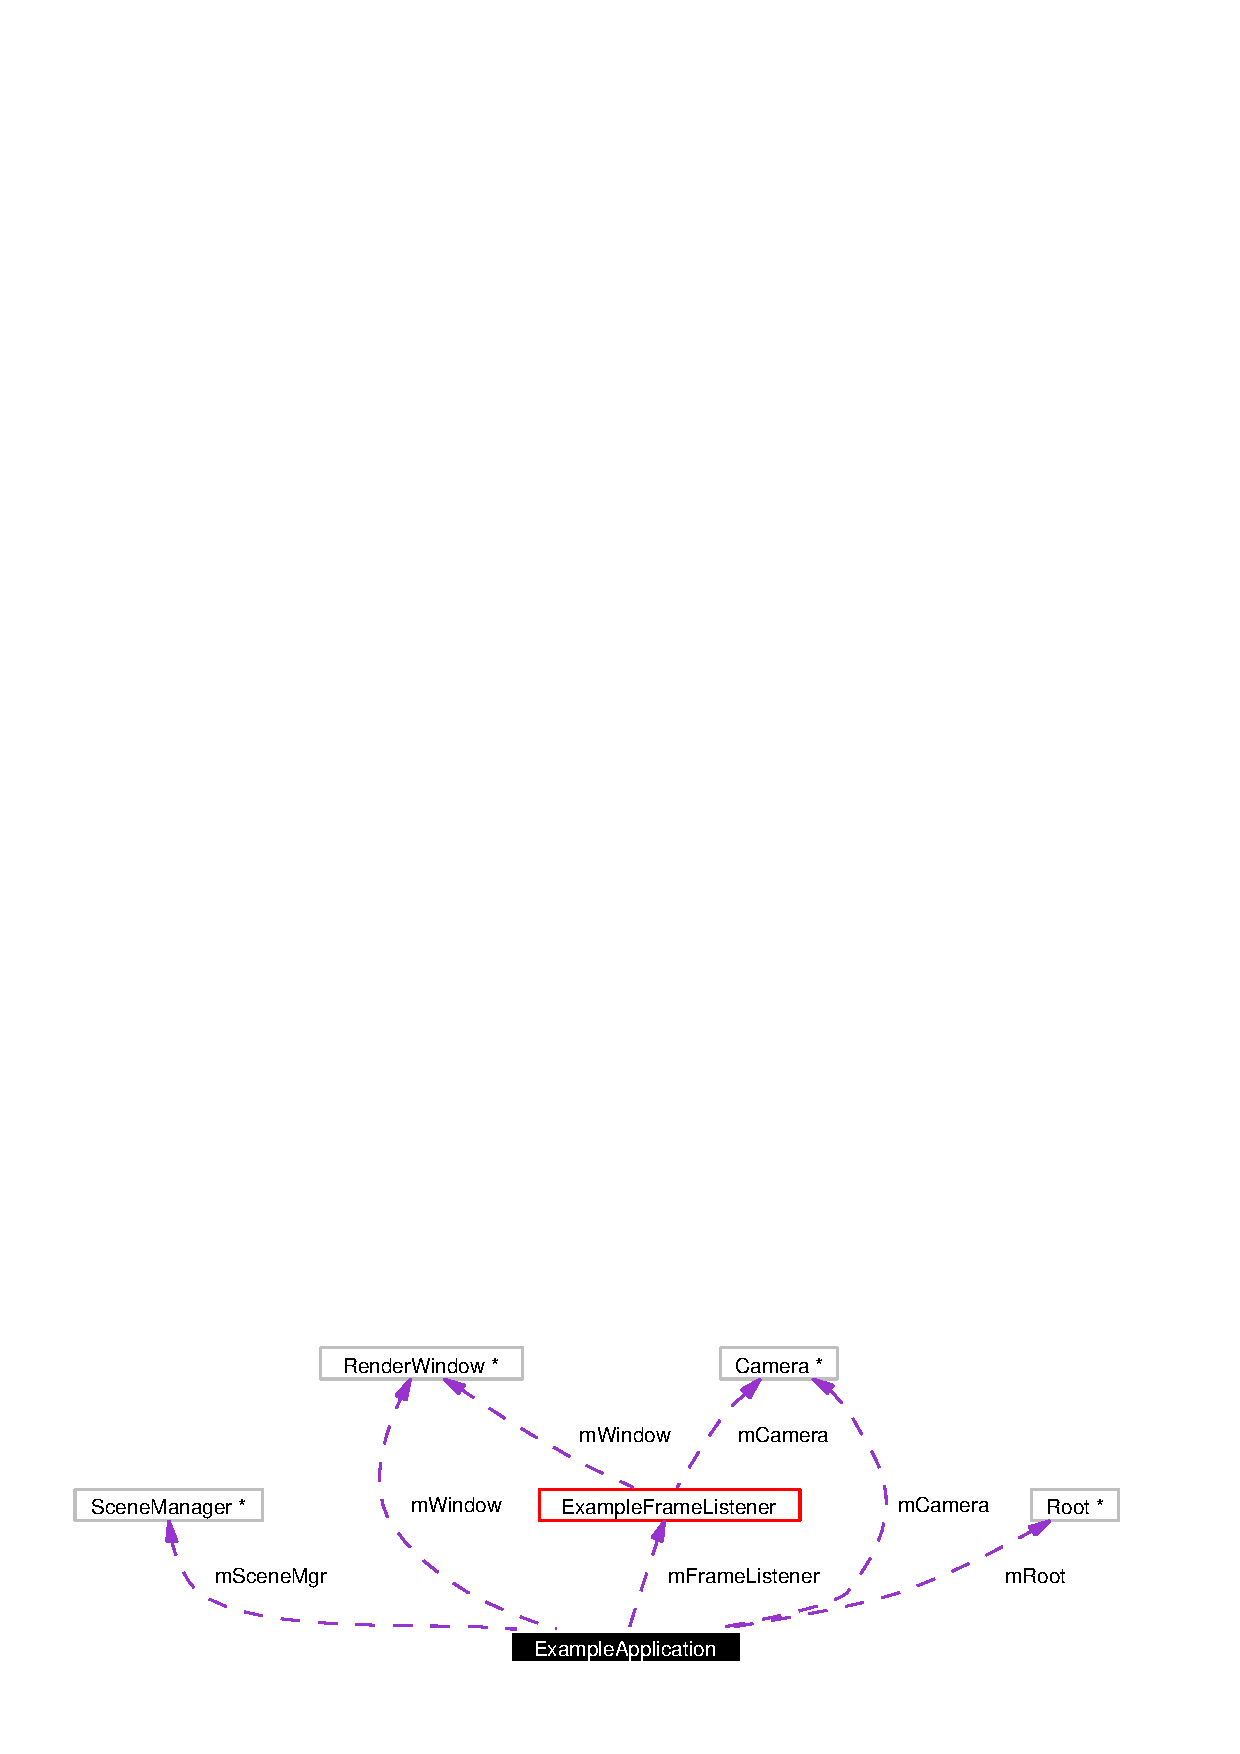
\includegraphics[width=280pt]{classExampleApplication__coll__graph}
\end{center}
\end{figure}
\subsection*{Public Member Functions}
\begin{CompactItemize}
\item 
{\bf Example\-Application} ()
\begin{CompactList}\small\item\em Standard constructor. \item\end{CompactList}\item 
void {\bf go} (int res\-X, int res\-Y)
\begin{CompactList}\small\item\em Start the example. \item\end{CompactList}\item 
{\bf $\sim$Example\-Application} ()
\begin{CompactList}\small\item\em Standard destructor. \item\end{CompactList}\item 
bool {\bf configure} (int res\-X, int res\-Y)
\item 
void {\bf choose\-Scene\-Manager} (void)
\item 
void {\bf create\-Camera} (void)
\item 
bool {\bf manual\-Initialize} (const String \&desired\-Renderer, int res\-X, int res\-Y)
\item 
void {\bf create\-Frame\-Listener} (void)
\item 
void {\bf create\-Scene} (void)
\item 
virtual void {\bf create\-Viewports} (void)
\item 
virtual void {\bf setup\-Resources} (void)
\begin{CompactList}\small\item\em Method which will define the source of resources (other than current folder). \item\end{CompactList}\end{CompactItemize}
\subsection*{Public Attributes}
\begin{CompactItemize}
\item 
Root $\ast$ {\bf m\-Root}
\item 
Camera $\ast$ {\bf m\-Camera}
\item 
Scene\-Manager $\ast$ {\bf m\-Scene\-Mgr}
\item 
{\bf Example\-Frame\-Listener} $\ast$ {\bf m\-Frame\-Listener}
\item 
Render\-Window $\ast$ {\bf m\-Window}
\end{CompactItemize}


\subsection{Detailed Description}
Base class which manages the standard startup of an {\bf Ogre}{\rm (p.\,\pageref{namespaceOgre})} application. Designed to be subclassed for specific examples if required. 



\subsection{Constructor \& Destructor Documentation}
\index{ExampleApplication@{Example\-Application}!ExampleApplication@{ExampleApplication}}
\index{ExampleApplication@{ExampleApplication}!ExampleApplication@{Example\-Application}}
\subsubsection{\setlength{\rightskip}{0pt plus 5cm}Example\-Application::Example\-Application ()\hspace{0.3cm}{\tt  [inline]}}\label{classExampleApplication_a0}


Standard constructor. 

\index{ExampleApplication@{Example\-Application}!~ExampleApplication@{$\sim$ExampleApplication}}
\index{~ExampleApplication@{$\sim$ExampleApplication}!ExampleApplication@{Example\-Application}}
\subsubsection{\setlength{\rightskip}{0pt plus 5cm}Example\-Application::$\sim${\bf Example\-Application} ()\hspace{0.3cm}{\tt  [inline]}}\label{classExampleApplication_a2}


Standard destructor. 



\subsection{Member Function Documentation}
\index{ExampleApplication@{Example\-Application}!chooseSceneManager@{chooseSceneManager}}
\index{chooseSceneManager@{chooseSceneManager}!ExampleApplication@{Example\-Application}}
\subsubsection{\setlength{\rightskip}{0pt plus 5cm}void Example\-Application::choose\-Scene\-Manager (void)\hspace{0.3cm}{\tt  [inline]}}\label{classExampleApplication_a4}


\index{ExampleApplication@{Example\-Application}!configure@{configure}}
\index{configure@{configure}!ExampleApplication@{Example\-Application}}
\subsubsection{\setlength{\rightskip}{0pt plus 5cm}bool Example\-Application::configure (int {\em res\-X}, int {\em res\-Y})\hspace{0.3cm}{\tt  [inline]}}\label{classExampleApplication_a3}


Configures the application - returns false if the user chooses to abandon configuration. \index{ExampleApplication@{Example\-Application}!createCamera@{createCamera}}
\index{createCamera@{createCamera}!ExampleApplication@{Example\-Application}}
\subsubsection{\setlength{\rightskip}{0pt plus 5cm}void Example\-Application::create\-Camera (void)\hspace{0.3cm}{\tt  [inline]}}\label{classExampleApplication_a5}


\index{ExampleApplication@{Example\-Application}!createFrameListener@{createFrameListener}}
\index{createFrameListener@{createFrameListener}!ExampleApplication@{Example\-Application}}
\subsubsection{\setlength{\rightskip}{0pt plus 5cm}void Example\-Application::create\-Frame\-Listener (void)\hspace{0.3cm}{\tt  [inline]}}\label{classExampleApplication_a7}


\index{ExampleApplication@{Example\-Application}!createScene@{createScene}}
\index{createScene@{createScene}!ExampleApplication@{Example\-Application}}
\subsubsection{\setlength{\rightskip}{0pt plus 5cm}void Example\-Application::create\-Scene (void)\hspace{0.3cm}{\tt  [inline]}}\label{classExampleApplication_a8}


\index{ExampleApplication@{Example\-Application}!createViewports@{createViewports}}
\index{createViewports@{createViewports}!ExampleApplication@{Example\-Application}}
\subsubsection{\setlength{\rightskip}{0pt plus 5cm}virtual void Example\-Application::create\-Viewports (void)\hspace{0.3cm}{\tt  [inline, virtual]}}\label{classExampleApplication_a9}


\index{ExampleApplication@{Example\-Application}!go@{go}}
\index{go@{go}!ExampleApplication@{Example\-Application}}
\subsubsection{\setlength{\rightskip}{0pt plus 5cm}void Example\-Application::go (int {\em res\-X}, int {\em res\-Y})\hspace{0.3cm}{\tt  [inline]}}\label{classExampleApplication_a1}


Start the example. 

\index{ExampleApplication@{Example\-Application}!manualInitialize@{manualInitialize}}
\index{manualInitialize@{manualInitialize}!ExampleApplication@{Example\-Application}}
\subsubsection{\setlength{\rightskip}{0pt plus 5cm}bool Example\-Application::manual\-Initialize (const String \& {\em desired\-Renderer}, int {\em res\-X}, int {\em res\-Y})\hspace{0.3cm}{\tt  [inline]}}\label{classExampleApplication_a6}


\index{ExampleApplication@{Example\-Application}!setupResources@{setupResources}}
\index{setupResources@{setupResources}!ExampleApplication@{Example\-Application}}
\subsubsection{\setlength{\rightskip}{0pt plus 5cm}virtual void Example\-Application::setup\-Resources (void)\hspace{0.3cm}{\tt  [inline, virtual]}}\label{classExampleApplication_a10}


Method which will define the source of resources (other than current folder). 



\subsection{Member Data Documentation}
\index{ExampleApplication@{Example\-Application}!mCamera@{mCamera}}
\index{mCamera@{mCamera}!ExampleApplication@{Example\-Application}}
\subsubsection{\setlength{\rightskip}{0pt plus 5cm}Camera$\ast$ {\bf Example\-Application::m\-Camera}}\label{classExampleApplication_o1}


\index{ExampleApplication@{Example\-Application}!mFrameListener@{mFrameListener}}
\index{mFrameListener@{mFrameListener}!ExampleApplication@{Example\-Application}}
\subsubsection{\setlength{\rightskip}{0pt plus 5cm}{\bf Example\-Frame\-Listener}$\ast$ {\bf Example\-Application::m\-Frame\-Listener}}\label{classExampleApplication_o3}


\index{ExampleApplication@{Example\-Application}!mRoot@{mRoot}}
\index{mRoot@{mRoot}!ExampleApplication@{Example\-Application}}
\subsubsection{\setlength{\rightskip}{0pt plus 5cm}Root$\ast$ {\bf Example\-Application::m\-Root}}\label{classExampleApplication_o0}


\index{ExampleApplication@{Example\-Application}!mSceneMgr@{mSceneMgr}}
\index{mSceneMgr@{mSceneMgr}!ExampleApplication@{Example\-Application}}
\subsubsection{\setlength{\rightskip}{0pt plus 5cm}Scene\-Manager$\ast$ {\bf Example\-Application::m\-Scene\-Mgr}}\label{classExampleApplication_o2}


\index{ExampleApplication@{Example\-Application}!mWindow@{mWindow}}
\index{mWindow@{mWindow}!ExampleApplication@{Example\-Application}}
\subsubsection{\setlength{\rightskip}{0pt plus 5cm}Render\-Window$\ast$ {\bf Example\-Application::m\-Window}}\label{classExampleApplication_o4}




The documentation for this class was generated from the following file:\begin{CompactItemize}
\item 
src/graphics/{\bf Example\-Application.h}\end{CompactItemize}
